% !TeX root = ../main.tex
\chapter{Theoretical background}
\label{chap:background}
In this chapter we want to provide with an overview on the general theoretical framework that supports this work, and introduce the main concepts for the successive parts. Each section in this chapter is, by no means, meant as an exhaustive treatment. The description will be quite conceptual, rather than technical, and aims at recalling the main ideas and fix conventions. We ask the reader to consult appropriate references,  which will be given in the corresponding sections, for a more detailed treatment of the topics. \\

\section{The renormalisation group}
\label{sec:RG}
Landau's mean field approach to study phase transition \cite{Landau:1937obd} gained wide popularity in the 1930's and 40's, since it was able to describe critical properties of many systems and it provided inspiration for the later Landau-Ginzburg theory of superconductivity \cite{ginzburg}. Thus, it was soon proved to be inaccurate to predict some experimentally well proven properties of certain systems near their critical point \cite{Cao:1999pw}. This is because, beeing a mean field theory, it did not take into account the role of spatial fluctuations.
The idea of block-spin transformation, systematically developed by Kadanoff \cite{PhysicsPhysiqueFizika_2_263}, made a big step towards a deeper understanding of the scaling behaviour, and posed the basis for the later work of Wilson \cite{WilsonRG1,WilsonRG2,WilsonFisher}, which still constitutes the basis for modern approaches to renormalisation in field theory and statistical physics.\\

\subsection{Block-spin RG}
\label{sec:blockspin}
\begin{figure}
    \centering 
    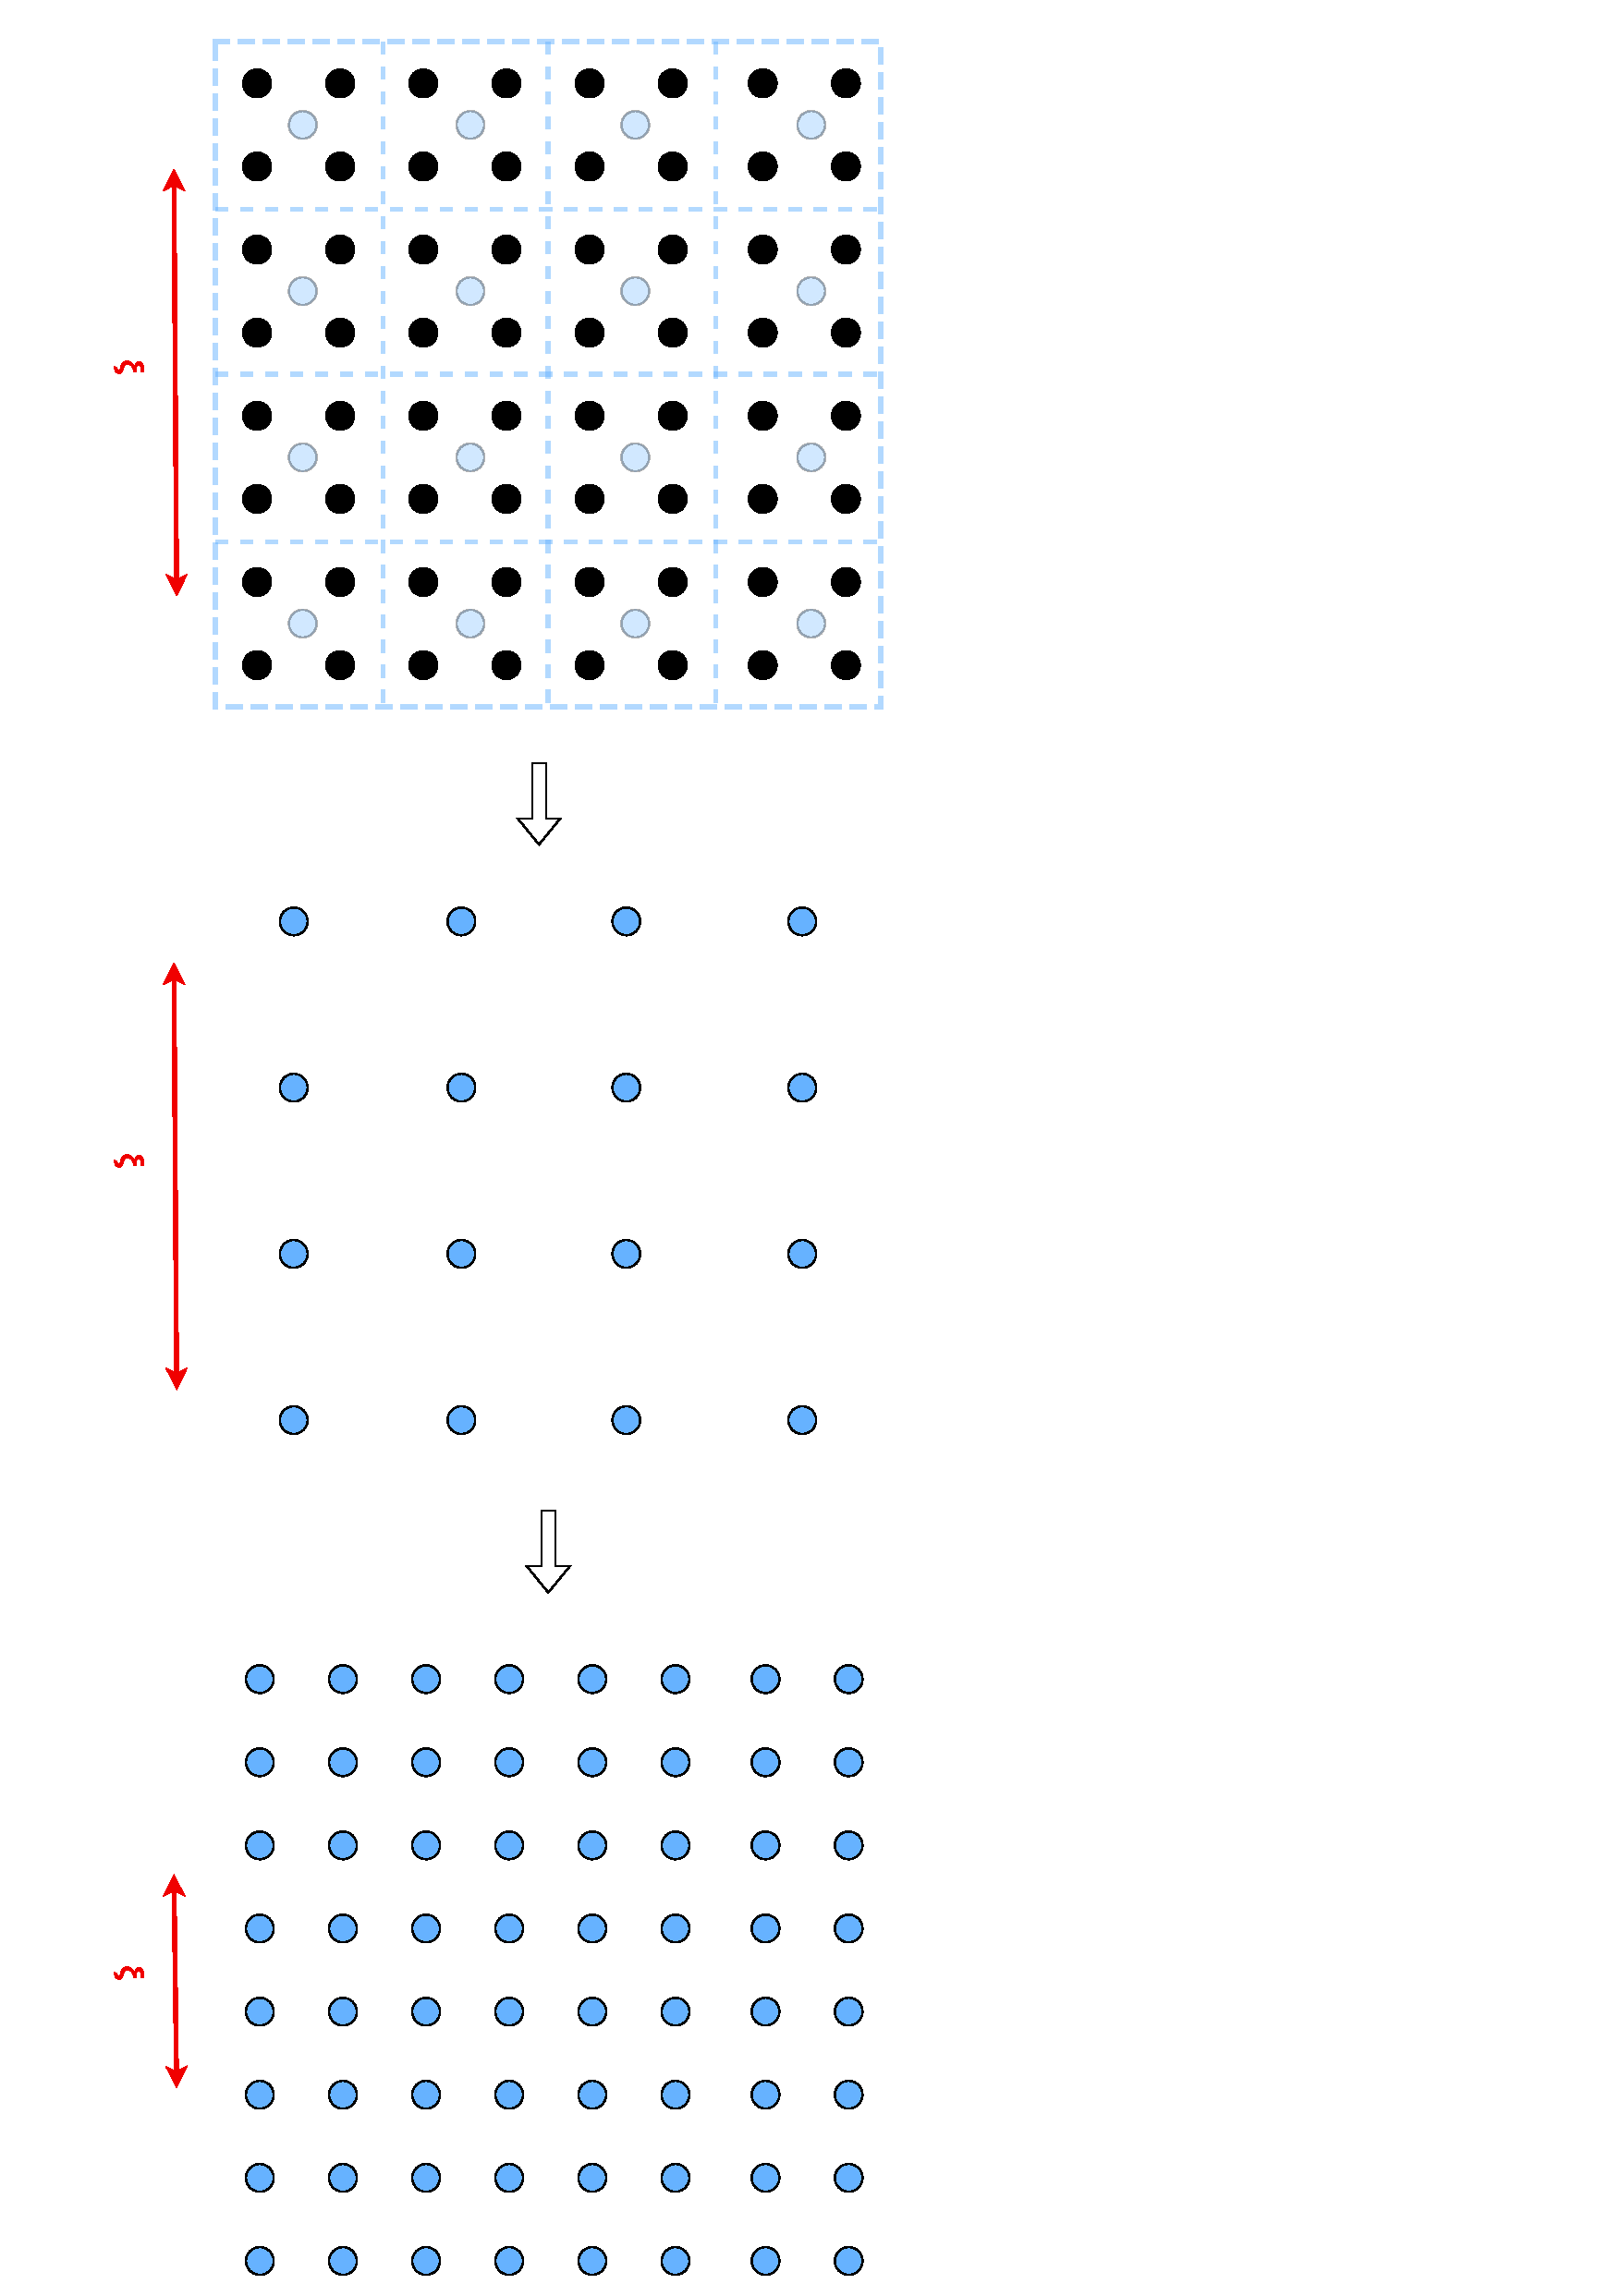
\includegraphics[angle=90,scale=0.34]{figures/blockspin.pdf}
    \caption[Block-spin transformation]{The two steps of the block-spin transformation. The black dots indicate the original field $\phi$, while the blue dots indicate the coarse-grained field $\bar \phi$.}
    \label{fig:blockin_first}
\end{figure}
To illustrate the idea, let us consider a set of spins whose magnetisation is described by a function $\phi(x)$. The spins are located on a discrete lattice $\mathscr{L}$ with spacing $a$, so that the function assumes values only at such sites $\phi(x_i) = \phi_i \neq 0 \Leftrightarrow x_i \in \mathscr{L}$. Suppose then that their interaction is described by a certain action $S[\phi]$ and a partition function
\begin{equation*}
    Z=\sum_{\phi} \mathrm{e}^{-S[\phi]}.
\end{equation*}
We now want to introduce a coarse-grained (or blocked) field $\bar\phi$ within a spacetime cell of volume $\mathcal{V}$. Such a coarse grained field can be defined, for example, as an average over the spins within the cell $\mathcal{V}$. If the spins can only be $0$ or $1$ like in a Ising model, then we might opt for a majority rule \cite{cardy_1996}.
We now want to find a new action $S_b$ such that 
\begin{equation}
    Z=\sum_{\phi} \mathrm{e}^{-S(\phi)}= \sum_{\bar\phi} \mathrm{e}^{-S_b\left(\bar\phi\right)}.
    \label{eq:blocked_action}
\end{equation}
Suppose for the moment that such $S_b$ has been found. The coarse-graining procedure comes with a loss of resolution since the spacing is changed $a \to 2a$. Hence one can rescale distances and momenta in the new action via $a \to a/2, p \to 2p$ and then compare the result with the initial action. This constitutes the second step of the block-spin transformation. \\
The whole procedure can be iterated multiple times, and can be thought as a zoom-out with a corresponding coarse graining, in order to describe the system in terms of the relevant scales as pictured in figure \ref{fig:blockin_first}. As made clear in the picture, the physical correlation length is reduced by the block-spin step, since the description is now in terms of the coarse field $\bar\phi$. 
There are only two exceptions for this, either the correlation length is zero, or infinite. The latter case represents a fixed-point of the RG, and the system exhibits scale invriance. \\
Note that the condition \eqref{eq:blocked_action} is non-trivial. One can, in principle, build an ad-hoc action that fulfills the condition, but it is complicated, since $S_b$ can be also be very different from $S$. For example, if the action $S[\phi]$ contains only nearest-neighbour interactions, the new action $S'[\bar\phi]$ can contain higher order interactions such as nearest-to-nearest neighbour, or even more.  In principle, all the terms compatible with the original symmetries are allowed, and one has often to rely on some approximations. For example, if one is interested in long range properties of the system, and the volume $V$ is sufficiently small, one can assume 
the functional form of the action $S$ to remain approximately the same, with the the only change due to the dimensional rescaling of dimensionful quantities mentioned above. Thus, as the procedure is iterated and the correlation length scale is approached, one has to take account higher order interactions. For an example of the explicit construction of the RG for an Ising model, see \cite{cardy_1996}.

\subsection{Wilsonian RG}
\label{sec:wilson_rg}
The Wilsonian picture of renormalisation \cite{WilsonRG1,WilsonRG2} is formulated in momentum space and in general is more suitable for theories in the continuum.\\
The idea is that a physical theory observed a energy scale $\Lambda$ can be seen as an effective theory of a more fundamental one, defined at scale $\Lambda_0 > \Lambda$. \\
To see how this can happen, let us consider a theory defined by the action $S[\phi]$ scale $\Lambda_0$, and let us split the field as 
\begin{equation*} 
    \phi = \bar\phi + \varphi
\end{equation*} 
where $\bar\phi$ are fields with momenta $p^2 \leq \Lambda^2$ and $\varphi$ are fields with $\Lambda^2 < p^2 \leq \Lambda_0^{2}$. \\
This allows to split the action as
\begin{equation*} 
    [\bar\phi + \varphi] = S_{\Lambda}[\bar\phi] + \delta S[\bar\phi, \varphi]
\end{equation*}
including all the dependence on $\varphi$ in $\delta S[\bar\phi, \varphi]$. \\
The path integral can be rewritten as
\begin{equation*}
    \begin{aligned}
        Z = \int D\phi \, e^{-S[\phi]} &= \int D\bar\phi_{\Lambda} \, e^{-S_{\Lambda}[\phi]} \int D\varphi  \, e^{-\delta S[\phi, \varphi]}  \\
        &= \int D\bar\phi_{\Lambda} \, e^{-S_{\Lambda}[\bar\phi] - S_\text{UV}[\bar\phi]}\\
        &= \int D\bar\phi_{\Lambda} \, e^{-S_{\Lambda}^\text{eff}[\bar\phi]},
    \end{aligned}
\end{equation*}
where 
\begin{equation*}
    S_{\Lambda}^\text{eff} = S_{\Lambda}[\bar\phi] + S_\text{UV}[\bar\phi], \qquad  S_\text{UV}[\bar\phi] = -\log\left( \int D\varphi \, e^{-S_{\Lambda}[\phi, \varphi]}\right).
\end{equation*}
$ S_\text{UV}[\bar\phi]$ encodes all the information of UV modes with $\Lambda^2 < p^2 \leq \Lambda_0^2$. \\
The action $S_{\Lambda}[\bar\phi]$ has the same functional form of the initial action $S[\phi]$, but it is now defined only for fields with momenta $p^2 \leq \Lambda^{2}$. Instead, $S^\text{eff}_\Lambda[\bar\phi]$ constitutes an effective description of the original theory at scale $\Lambda$ and depends only on degrees of freedom with $p^2 \leq \Lambda^2$. \\
One can then operate a rescaling of distances and momenta to complete the Wilson RG step, according to the parameter 
\begin{equation*}
    s^2 = \Lambda^2 / \Lambda_0^2.
\end{equation*}
If, for example, $d_g$ is the energy dimension of a coupling $g$ in the action, then the rescaling transformation causes 
\begin{equation*} 
    g \to s^{d_g} \, g.
\end{equation*}
The same applies to the fields and other dimensionful quantities. If the corrections from $S_\text{UV}$ are negligible, such as for high cutoff $\Lambda \approx \Lambda_0$, then this is the only contribution to the change in the couplings and fields due to the Wilson step. More in general, for higher order iterations of the procedure, the couplings' dependence on $s$ is caputered by the $\beta$-functions 
\begin{equation*}
    \beta_g = \frac{d}{ds} \, g(s).
\end{equation*}
A full treatment of RG is out of scope here and we ask the reader to consult more appropriate references fore more details \cite{Peskin:1995ev}. \\~\\
At this point, one can clearly see the analogy with the block-spin transformation introduced in the previous section. Performing the integral over high momenta modes
can be thought as performing averages (coarse graining) over neighbours. This causes a loss of resolution which can be recovered by rescaling distances and momenta. The rescaling is essential for a description of fixed points, since it can be pictured as a zoom-out. \\
Therefore, the philosophy of Kadanoff and Wilson approaches was that the blocking transformation reduces the complexity of many-body systems by systematically reducing the number of degrees of freedom being taken into account, without changing the physical content of the
theory \cite{WILSON197475,carosso2020novel}. \\~\\
We want to conclude this section by mentioning that the splitting of the action can be done by writing
\begin{equation*}
    S^\text{eff}_\Lambda[\bar\phi] = S[\phi] + \Delta S_{\Lambda}^{(\mathrm{IR})}[\bar\phi],
\end{equation*}
where $\Delta S_{\Lambda}^{(\mathrm{IR})}[\hat{\phi}]$ is a regulating function which typically assumes the form
\begin{equation} 
    \Delta S_{\Lambda}^{(\mathrm{IR})}[\bar\phi] = \frac{1}{2} \int \frac{\mathrm{d}^d p}{(2 \pi)^d} \bar\phi(-p) \ \Lambda^2 \, \left(\frac{1}{r_{\Lambda}(p^2)}-1\right) \ \bar\phi(p),
\end{equation}
For a sharp momentum cutoff one has
\begin{equation*}
    r_{\Lambda}(p^2) = \theta\left(p^2-\Lambda^2\right).
\end{equation*}
This result will allow for a deep connection between coloured stochastic quantisation and the functional renormalisation group, the latter describing the functional dependence of $S_\Lambda^\text{eff}[\bar\phi]$ on the cutoff scale $\Lambda$ \textcolor{red}{citationsssss}.


\section{Lattice QFT and the continuum limit}
\label{sec:lattice_continuum_}
The starting set up is the euclidean formulation of quantum field theory, where one typically defines a path integral $Z$, which, for a general scalar field $\phi(x)$ and a fermion field $\psi(x)$, assumes the form
\begin{equation}
    Z = \int \mathcal{D}\phi\mathcal{D}\psi\mathcal{D}\bar\psi \ e^{-S[\phi, \psi, \bar\psi]}, \qquad \mathcal{D}\xi = \prod_x d\xi_x, \quad \xi \in \{\phi, \psi, \bar\psi\},
    \label{eq:path_integral_generic}
\end{equation}
and correlation functions are computed via
\begin{equation*}
        \left\langle \xi_{x_1} \dots \xi_{x_n}  \right\rangle = \frac{1}{Z} \int \mathcal{D}\phi\mathcal{D}\psi\mathcal{D}\bar\psi \ \xi_{x_1} \dots \xi_{x_n} \ e^{-S[\phi, \psi, \bar\psi]}, \qquad \xi_{x_i} \in \{\phi_{x_i}, \psi_{x_i}, \bar\psi_{x_i}\}. \\
\end{equation*}
Let us then consider a lattice $\mathscr{L}$, with spacing $a$, and $N_\mu$ points in each spacetime direction $\mu$, hence a physical length $L_\mu = N_\mu \, a$.
For simplicity we restricted here to a scalar field $\phi$ and we will recall fermionic properties only when relevant, but what follows has general validity. 
The action and the path integral measure are now taken over discrete quantities 
\begin{equation*}
    \begin{aligned}
	    S = \int d^dx \, \mathcal{L}(\phi(x)) \qquad &\to \qquad S = a^d \sum_{n \in \mathscr{L}} \, \mathcal{L}(\phi(n)), \\
        \prod_{x} d\phi(x) \qquad &\to  \qquad \prod_{n \in \mathscr{L}} d\phi(n),
    \end{aligned}
\end{equation*}
where $\mathcal{L}(\phi)$ is the Lagrangian density function.  \\
The path integral is hence
\begin{equation*}
    Z = \int \prod_n d\phi(n) \, e^{-S[\phi]},
\end{equation*}
and the probability of a field configuration $\phi$
\begin{equation}
    p(\phi) = \frac{1}{Z} \, e^{-S[\phi]}.
    \label{eq:probability_distribution_lattice}
\end{equation}
Expectation value of observables are computes as
\begin{equation}
    \expect{O(\phi)}  = \frac{1}{Z} \, \int \prod_n d\phi(n) \, O(\phi) \, e^{-S[\phi]}.
    \label{eq:expectation_value_lattice}
\end{equation}
In order to simulate a theory and perform the above sums one has to go to finite volumes and impose boundary conditions. In the space directions, we take periodic conditions 
\begin{equation*}
    \begin{aligned}
        \phi(t, \vec x) &= \phi(t, \vec x + \vec T), \\
        \psi(t, \vec x) &= \psi(t, \vec x + \vec T).
    \end{aligned}
\end{equation*}
Instead, a finite time extent is related to the temperature of the system \cite{le_bellac_1996,rothe_LGT} via
\begin{equation*}
    \beta = 1/T = 1/L_t,
\end{equation*}
and boundary conditions are chosen depending on the spin-statistic of the corresponding particles, namely periodic conditions for bosons, and anti-periodic for fermions
\begin{equation*}
    \begin{aligned}
        \phi(t, \vec x) &= \phi(t + T, \vec x) \qquad \text{bosons}, \\
        \psi(t, \vec x) &= -\psi(t + T, \vec x) \quad \text{fermions}.
    \end{aligned}
\end{equation*}
Such a formulation naturally brings a momentum cutoff $\Lambda = \pi/a$ since now all the momenta are restricted to the first Brilloune zone $p_\mu \in [-\pi/a, \pi/a]$. \\~\\
To compute observables one relies on Monte-Carlo methods to generate field configurations, sampling the distribution \eqref{eq:probability_distribution_lattice} and convergence to the statistical value given by \eqref{eq:expectation_value_lattice} is expected in the limit of infinite samples $N_\text{samp} \to \infty$. \\
To recover the continuum results, one has to take $V \to \infty, a \to 0$ \footnote{the order here is important, see for example \cite{seiler,friedli_velenik_2017}}, but this task cannot be done so straightforwardly.
Continuum limits of lattice theories are intimately connected to the existence of critical points. To see why this is the case, consider the dimensionless mass gap 
\begin{equation*}   
    \hat\xi = m \, a
\end{equation*} 
of a certain theory. The quantity $\xi$ is also called correlation length and it is related to the exponential decay of correlation functions between local observables measured
at different points on the lattice, as given by \textcolor{red}{add ref. eq.}\\
When taking the continuum limit we want $a \to 0$, while having a finite physical mass $m$. This implies that the correlation length $\hat \xi$ has to diverge: in the language of statistical physics, this is a second order phase transition. Of course to bring the system at its critical point, where such phase transition happens, one has to tune the bare parameters $g_0^i$ of the theory to their critical values $g_0^{i \, *}$. 
To do this, one should find the zeros of the lattice beta functions
\begin{equation*}
    \beta_g^\text{latt} = a \frac{d}{da} g(a) \overset{!}{=} 0, \qquad a = \pi/\Lambda.
\end{equation*}
As this is quite hard task to do on the lattice, one typically relies on some approximation schemes such as employing perturbative continuum beta functions. \\
In any case, from this description it should be clear that the spacing $a$ should not be treated as a free parameter in the continuum limit, but rather a dynamically determined quantity that depends on the couplings of the theory.\\~\\
Note that in the limit $a \to 0$, one has $\Lambda \to \infty$. If one's scope is to simulate an effective theory which is expected to hold only up to a scale $\Lambda_\text{phys}$, one must have $\Lambda \leq \Lambda_\text{phys}$, with a consequent lower bound on the lattice spacing $a \geq a_\text{phys} = \pi / \Lambda_\text{phys}$. \\ ~

\section{Stochastic quantisation}
\label{sec:stochastic_quantisation}
The idea of stochastic quantisation \cite{ParisiWu,Damgaard1987StochasticQuantization} is that Euclidean Quantum Field theory can be thought as a system in thermal equilibrium with a heat reservoir and hence described as a stochastic process via the Langevin equation. For this, one has to introduce a fictitious time variable $\tau$ that labels the state $\phi(\tau, x)$ of the system 
during the evolution. \\
\subsection{Standard stochastic quantisation}
Let us consider, for example, a scalar field $\phi$ with a Euclidean action $S[\phi]$ and the following Langevin equation
\begin{equation}
    \partial_\tau \phi(\tau, x) = - \frac{\delta S[\phi]}{\delta \phi (\tau, x)} + \eta (\tau, x),
    \label{eq:Langevin_scalar_full}
\end{equation}
where $K_{\phi}(\tau) \equiv -\delta S[\phi]/\delta \phi (\tau, x)$ is the drift term and $\eta (\tau, x)$ is a random white noise field assumed to be normally distributed
\begin{equation*}
    P(\eta) = \frac{\exp\left(-\frac{1}{4}\int_{\tau,x} \eta^2(\tau, x)\right)}{\int D\eta \exp\left(-\frac{1}{4}\int_{\tau,x} \eta^2(\tau,x)\right)},
\end{equation*} 
which, in particular, implies
\begin{equation}
    \expect{\eta(x,\tau)} = 0, \qquad \expect{\eta(x,\tau) \, \eta(x',\tau')} = 2 \, \delta(x - x') \, \delta (\tau - \tau').
    \label{eq:white_noise_definition}
\end{equation}
Stochastic average with respect to the measure $P(\eta)$ are computed via 
\begin{equation*}
    \expect{A(\eta)} = \int D\eta \, P(\eta) \, A(\eta).
\end{equation*}
In momentum space, \eqref{eq:white_noise_definition} becomes
\begin{equation}
    \begin{aligned}
        \expect{\eta(p,\tau)} &= \expect{\int_x e^{ipx}\eta(x,\tau)} = \int_x \expect{e^{ipx}\eta(x,\tau)} = 0, \\
        \expect{\eta(p,\tau)\eta(q,\tau')} &= \expect{\int_{xy} e^{ipx + iqy} \eta(x,\tau)\eta(y,\tau')} \\
        &= \int_{xy} e^{ipx + iqy} \expect{\eta(x,\tau)\eta(y,\tau')} \\
        &= 2 \, (2\pi)^2 \, \delta(p + q) \, \delta(\tau - \tau').
    \end{aligned}
    \label{eq:white_noise_definition_momentum}
\end{equation}
In absence of the noise term $\eta(\tau,x)$, equation \eqref{eq:Langevin_scalar_full} simply represents an evolution of the field towards the minimum of the action, and at equilibrium the field is constrained to $\partial_\tau \phi(x,\tau) = 0 = \delta S[\phi]/\delta \phi (\tau, x)$, namely to the classical equations of motion.\\
For any observable $O$, which is function of the field, one has, for fixed time $\tau$,
\begin{equation*}
    \expect{O(\phi(\tau))} = \int D\eta \, P(\eta) \, O(\phi(\tau)),
\end{equation*}
from which it follows straightforwardly using the Langevin equation and $\expect{\eta} = 0$
\begin{equation*}
    \frac{d}{d\tau} \expect{O(\phi(\tau))} = \expect{\frac{\delta O}{\delta \phi(\tau, x)} \ \partial_\tau \phi(\tau, x)} = -\expect{\frac{\delta O}{\delta \phi}(\tau, x) \ \frac{\delta S}{\delta \phi(\tau, x)}}.
\end{equation*}
It follows trivially that for $O(\phi(\tau)) = \phi(\tau, x)$
\begin{equation*}
        \frac{d}{d\tau} \expect{\phi(\tau, x)} = -\expect{\frac{\delta S}{\delta \phi(\tau, x)}} \quad \underset{Equilibrium}{\Longrightarrow} \quad \expect{\frac{\delta S}{\delta \phi(\tau, x)}} = 0.
\end{equation*}
This also provides a consistency check for the correct implementation of the simulation, since the drift $K_\phi = -\delta S / \delta \phi$ is computed numerically during the evolution. \\
More generally, one can derive a correspondent Fokker-Planck equation \cite{gardiner}, which can be proven to have a stationary distribution if the action is bounded from below, given by \cite{Damgaard1987StochasticQuantization}
\begin{equation}
    \mathcal{P}(\phi) = \frac{1}{Z} \, \exp\left(-S[\phi]\right).
    \label{eq:probability_field_configuration_full}
\end{equation}
This allows one to compute correlation functions as moments of the  probability distribution \eqref{eq:probability_field_configuration_full}. In particular, one has 
\begin{equation}
    \expect{O}_{P(\eta)} = \expect{O}_{\mathcal{P}(\phi)} \equiv \expect{O}.
    \label{eq:expectation_observables}
\end{equation}

\subsection{Stochastic quantisation with coloured noise}
\label{sec:coloured_noise}
In the stochastic quantisation procedure the noise which accounts for the quantum fluctuations of the theory is assumed to be white, as defined in equations \eqref{eq:white_noise_definition}, \eqref{eq:white_noise_definition_momentum}. 
We now want to examine the dynamics in presence of a coloured noise, writing the Langevin equation as
\begin{equation*}
    \partial_\tau \phi(x, \tau) = - \frac{\delta S[\phi]}{\delta \phi (\tau, x)} + \eta_\text{col}(x, \tau),
    \label{eq:Langevin_scalar_regularised}
\end{equation*}
with $\eta_\text{col}(x,\tau) = r_\Lambda(x) \, \eta(x,\tau)$. In particular, here we restrict to the regulating function defined as a sharp cutoff in momentum space
\begin{equation}
    r_\Lambda(p) = \theta(\Lambda^2 - p^2),
    \label{eq:regulator}
\end{equation}
and we invite the reader to consult \cite{Pawlowski2017CoolingNoise} for a discussion of other regulating functions. \\
The noise field in momentum space is then
\begin{equation*}
    \begin{aligned}
        \eta_\text{col}(p, \tau) &= \mathcal{F}[\eta_\text{col}(x,\tau)] = \mathcal{F}[r_\Lambda(x,\tau) \eta(x,\tau)] = \mathcal{F}[r_\Lambda(x,\tau)] \star \mathcal{F}[\eta(x,\tau)] \\
        &= \theta(\Lambda^2 - p^2)  \, \eta(p, \tau).
    \end{aligned}
\end{equation*}
where $\mathcal{F}$ indicates the Fourier transform and $\star$ the convolution product. \\
An interesting quantity to look at is the position-space noise correlation function
\begin{equation}
    \begin{aligned}
        C_{\eta}(x,\tau,y,\tau') &= \left\langle\eta_\text{col}(x,\tau) \, \eta_\text{col}(y,\tau')\right\rangle \\
        &= \frac{1}{(2\pi)^{4}} \int D\eta \, P(\eta) \left[\int_{p,q} e^{-ipx-iqy }\eta_\text{col}(p,\tau) \, \eta_\text{col}(q,\tau')\right] \\
        &= \frac{1}{(2\pi)^{4}} \int_{p,q} e^{-ipx-iqy } \int D\eta \left[ P(\eta) \, \eta(p,\tau) \, \eta(q,\tau') \right] \\
        &\qquad\times \theta(\Lambda^2 - p^2) \, \theta(\Lambda^2 - q^2)  \\
        &= \frac{2}{(2\pi)^{2}} \int_{p,q} e^{-ipx-iqy} \, \delta(p+q) \, \theta(\Lambda^2 - p^2) \, \theta(\Lambda^2 - q^2) \, \delta(\tau - \tau') \\
        &= \frac{2}{(2\pi)^{2}} \int_{p} e^{-ip(x-y)} \, \theta(\Lambda^2 - p^2) = \frac{1}{\pi} \, \int_0^\Lambda \, d\omega \, \omega \, J_0(\omega |x-y|),
    \end{aligned}
    \label{eq:coloured_noise_correlation}
\end{equation}
where $J_0(x)$ is a Bessel function of the first order. The integral in the last line is computed numerically as a function of $d=|x-y|$ and reported in figure \ref{fig:bessel} for three different values of the cutoff $\Lambda_1 < \Lambda_2 < \Lambda_3$. This shows nicely that for $|x-y| \ll 1/\Lambda$ the noise is now correlated, while for $|x-y| \gg 1/\Lambda$ the correlation function vanishes, as in the white noise case. In other words, only the short-length behaviour of the system is affected by the introduction of such a regulating term, as one could expect.\\~\\
\begin{figure}
    \centering
    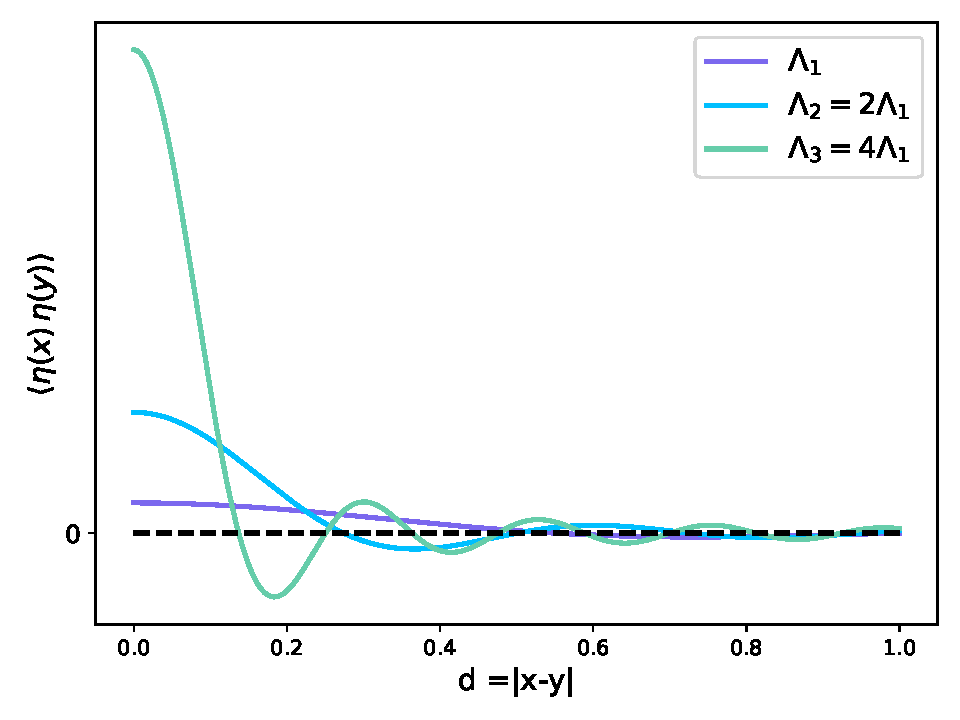
\includegraphics[scale=0.6]{figures/bessel.pdf}
    \caption[Correlated noise]{Noise correlation as a function of $d=|x-y|$ for three different values of the cutoff $\Lambda_1 < \Lambda_2 < \Lambda_3$, in arbitrary units. The plot is qualitative, but shows clearly that with a regulated noise, only the short-distance behaviour is affected.}
    \label{fig:bessel}
\end{figure}
Another intuitive and interesting aspect of the dynamics in the presence of coloured noise can be deduce by looking at the field expression in terms of the retarded Langevin Green function \cite{Damgaard1987StochasticQuantization}, which is here not derived, but reported from \cite{Pawlowski2017CoolingNoise}
\begin{equation*}
        \phi(x, \tau) = \int_{x^{\prime}} \int_{-\infty}^\tau \mathrm{d} \tau^{\prime} G\left(x-x^{\prime}, \tau-\tau^{\prime}\right) \, \left[r_{\Lambda}\left(\Delta_x\right) \eta\left(x, \tau^{\prime}\right)-\frac{\delta S}{\delta \phi}|_{p=0} \, \phi\left(x^{\prime}, \tau\right)\right],
\end{equation*}
where
\begin{equation*}
    G\left(x-x^{\prime}, \tau-\tau^{\prime}\right) =\theta\left(\tau-\tau^{\prime}\right) \int_p \mathrm{e}^{-i p \cdot\left(x-x^{\prime}\right)} \mathrm{e}^{-\left(\tau-\tau^{\prime}\right)\left(p^2+m^2\right)}.
\end{equation*}
By looking at the first term in the square bracket, one can conclude that there is no propagation of modes with momentum $p^2\geq \Lambda^2$ due to the noise term, but one can still have contribution from modes $p^2 > \Lambda^2$ from the second term, which corresponds to the deterministic part of the equations of motion. Stated differently, UV quantum fluctuations with $p^2 > \Lambda^2$ are removed from the dynamics of $\phi$, but still contribute classically. \\~\\
Generally speaking, the stationary distribution probability of the regulated stochastic process is given by \cite{Pawlowski2017CoolingNoise}
\begin{equation}
    \mathcal{P}_\Lambda(\phi) = \frac{1}{Z} \, \exp\left(-S_\Lambda[\phi]\right) = \frac{1}{Z} \, \exp\left(-(S[\phi] + \Delta S_\Lambda[\phi])\right),
    \label{eq:probability_field_configuration_regularised}
\end{equation}
where the correction term $\Delta S_\Lambda[\phi]$, reads, for a regulator $r_\Lambda(p^2)$,
\begin{equation*}
        \Delta S_{\Lambda}[\phi]=\frac{1}{2} \int_p \phi_p \, \Lambda^2\left(\frac{1}{r_{\Lambda}\left(p^2\right)}-1\right) \, \phi_{-p}.
\end{equation*}
\textcolor{red}{at this point mention that this is the stationary pdf that one gets with frg for sharp cutoff, and cite some papers.}

\section{Chiral symmetry}
\label{sec:chiral_symmetry}
In this section we want to introduce chiral symmetry and its breaking, both in the continuum and on the lattice. \\
It is useful to adopt the notation 
\begin{equation*}
    \psi = (\psi^{(1)}, \dots, \psi^{(N_f)}).
\end{equation*} 
We then introduce left-handed and right-handed spinors
\begin{equation*}
	\psi_L = (1-\gamma_5) \, \psi, \qquad \psi_R = (1+\gamma_5) \, \psi,
\end{equation*}
for which
\begin{equation*}
	\psi = \frac{(1-\gamma_5)}{2} \psi + \frac{(1+\gamma_5)}{2} \psi = \psi_L + \psi_R.
\end{equation*}


\subsection{Chiral symmetry in the continuum}

The free massless Dirac Lagrangian
\begin{equation} 
    \mathcal{L}_D = \bar\psi \slashed{\partial} \psi = \bar\psi_L \slashed{\partial} \psi_L + \bar\psi_R \slashed{\partial} \psi_R
\end{equation} 
is symmetric under the chiral group $SU(N_f) _L\times SU(N_f)_R$, namely
\begin{equation*}
	\begin{aligned}
		\psi_L(x) \to U_L\psi_L(x), &\qquad \bar\psi_L(x) \to \bar\psi_L(x) U_L^{\dagger}, \\
		\psi_R(x) \to U_R\psi_R(x), &\qquad \bar\psi_R(x) \to \bar\psi_R(x) U_R^{\dagger},
	\end{aligned}
\end{equation*}
for $U_L, U_R \in SU(N_f)$. \\
In terms of the full spinor $\psi$, the chiral symmetry can be written as 
\begin{equation*} 
    \psi \to M \, \psi, \qquad \bar\psi \to \bar\psi,
\end{equation*} 
where
\begin{equation*}
    M = e^{i(\theta_a \tau^a + \gamma_5 \beta_a\tau^a)}, \quad \tau^a \in su(N_f)
\end{equation*}
so that 
\begin{equation*} 
    SU(N_f) _L\times SU(N_f)_R \simeq SU(N_f)_V \times SU(N_f)_A.
\end{equation*}
$SU(N_f)_V$ is the isospin subgroup, characterised by $\beta_a =0$, and $SU(N_f)_A$ is the axial rotation subgroup, characterised by $\theta_a = 0$. \\
To be more precise, the full invariance group of the classical action is
\begin{equation*}
    SU(N_f)_L \times SU(N_f)_R \times U(1)_A \times U(1)_V,
\end{equation*}
where the axial and vector symmetry transformations are, respectively,
\begin{equation*}
        \psi \to e^{i\theta \gamma_5} \, \psi, \qquad \psi \to e^{i\theta} \, \psi.
\end{equation*} 
One can thus prove that axial symmetry is broken by quantum anomalies (see for example \cite{schwartz}), so that the symmetry in the quantum case is
\begin{equation*}
    SU(N_f)_L \times SU(N_f)_R \times U(1)_V.
\end{equation*}
If equal masses for each flavour are introduced, then the symmetry group reduces to the isospin subgroup, diagonal in flavour space
\begin{equation*}
    SU(N_f)_V \times U(1)_V.
\end{equation*}
Finally, if the fermions have different masses, the symmetry group reduces to 
\begin{equation*}
    \underbrace{U(1) \times \dots \times U(1)}_{N_f} \times U(1)_V.
\end{equation*}

\subsection{Chiral symmetry on the lattice}
The essence of chiral symmetry for fermions can be expressed as \cite{gattringer_LQCD}
\begin{equation}
    \left\{\gamma_5, D \right\} = 0
    \label{eq:chiral_symmetry}
\end{equation}
Implementing chiral symmetry on a finite-volume spacetime lattice, is a hard task. This is because, as proven by Nielsen and Ninomiya, one either has chiral symmetry on the lattice, or solves the doubling problem \textcolor{red}{citationsssss}. \\
In particular, the insertion of the Wilson term in the action, as shown in Appendix \ref{chap:AppendixB}, causes explicit breaking of the chiral symmetry. If one's goal is to study spontaneous symmetry breaking, this constitues a problem. 
Thus, many options have been proposed to circumvent the issue. As an example we mention the approach by Ginsparg and Wilson \textcolor{red}{citationsssss}, who proposed to modify the chiral symmetry condition \eqref{sec:chiral_symmetry} to 
\begin{equation*}
    \left\{\gamma_5, D \right\} = a \, D \gamma_5 D
\end{equation*}
The right hand-side of the equation vanishes in the continuum limit $a \to 0$. In this way, one can define chiral symmetry on the lattice remaining consistent in the continuum limit. This approach will not be pursued further and we ask the reader to consult 
appropriate references \cite{rothe_LGT,gattringer_LQCD} for a detailed treatment. \\
Our approach to study chiral symmetry will be discussed and motivated in section \ref{sec:chiral_PT}.

\section{Yukawa theory}
\label{sec:Yukawa_theory}

\subsection{Description of the model}
Let us consider the Yukawa theory defined by the action
\begin{equation}
\begin{aligned}
    S[\phi,\psi,\bar\psi] &= S_\phi[\phi] + S_\psi[\psi, \bar\psi] + S_\text{int}[\phi, \psi, \bar\psi], \\
     S_\phi[\phi] &= \int_x \phi_x \left(-\frac{\partial^2_x}{2} + \frac{m_\phi^2}{2}\right) \phi_x + \frac{\lambda}{4!} \, \phi_x^4, \\
     S_\psi[\psi, \bar\psi] &= \int_x \sum_{f=1}^{N_f} \bar \psi_x^{(f)} \left(\slashed{\partial}_x + m_q \right) \psi_x^{(f)}, \\
     S_\text{int}[\phi, \psi, \bar\psi] &= \int_x \sum_{f=1}^{N_f} g \, \bar \psi_x^{(f)} \, \phi_x \, \psi_x^{(f)}.
    \label{eq:full_action_continuum}
\end{aligned}
\end{equation}
One can see that the action is made of a scalar part $S_\phi[\phi]$, a fermionic part $S_\psi[\psi, \bar\psi]$ and a Yukawa interaction term $S_\text{int}[\phi, \psi, \bar\psi]$. \\
In pratice we will work with fixed number of flavours $N_f = 2$, but it is useful to keep track of $N_f$ and set it to its value when needed. \\
It is also convenient for later purposes to define the operators $K, D$ represented in position space as 
\begin{equation}
    \begin{aligned}
        K(x, y) &=  \left(-\partial^2_x + m_\phi^2\right) \ \delta(x,y), \\
        D(x, y) &= \left(\slashed{\partial}_x + m_q + g\phi \right) \ \delta(x,y),
    \end{aligned}
    \label{eq:definition_kinetic_terms_continuum_position}
\end{equation}
and in momentum space as
\begin{equation}
    \begin{aligned}
        \widetilde{K}(p, q) &=  \int_{x,y} e^{-ipx} \left(\partial^2_x + m_\phi^2\right) \ \delta(x,y) \ e^{iqy} = \left(\frac{p^2}{2} + \frac{m_\phi^2}{2}\right) \ \delta(p,q), \\
        \widetilde{D}(p, q) &= \int_{x,y} e^{-ipx} \left(\slashed{\partial}_x + m_q + g\phi \right) \ \delta(x,y) \ e^{iqy} = \left(\slashed{p}_x + m_q + g\phi \right) \ \delta(p,q).
    \end{aligned}
    \label{eq:definition_kinetic_terms_continuum_momentum}
\end{equation}
This allows one to rewrite the action as
\begin{equation*}
    S[\phi,\psi,\bar\psi] = \int_x \frac{1}{2} \, \phi_x \, K_{xx} \, \phi_x + \frac{\lambda}{4!} \, \phi_x^4 + \sum_{f=1}^{N_f} \bar\psi_x^{(f)} \, D_{xx} \, \psi_x^{(f)}.
\end{equation*}

\subsection{Chiral symmetry in the Yukawa model}
The action written in terms of $\psi_L, \psi_R$, reads
\begin{equation}
	S = S_\phi +  \int_x \left[\bar\psi_L \, D \, \psi_L + \bar\psi_R \, D \, \psi_R + (m_q + g\phi) \,  \left(\bar\psi_L\psi_R + \bar\psi_R\psi_L\right)\right].
	\label{eq:action_chirality_explicit}
\end{equation}
The action is not invariant under the full chiral group, but if $m_q = 0$ it is symmetric under the discrete chiral transformation
\begin{equation*}
    \begin{aligned}
        \phi &\to -\phi, \\
        \psi_L \to \gamma_5 \psi_L, &\qquad \bar\psi_L \to \bar\psi_L\gamma_5, \\
        \psi_R \to \gamma_5 \psi_R, &\qquad \bar\psi_R \to \bar\psi_R\gamma_5,
    \end{aligned}
\end{equation*}
typical of theories such as the Gross-Neveu model \textcolor{red}{citationsssss}. In order to generalise the model to the full chiral group, one has to consider an $O(4)$ scalar sector and interactions, since $O(4) \simeq SU(2) \times SU(2)$. Similar effective theories with such properties are, for example, 
the Nambu-Jona-Lasinio model and the Quark-Meson model \textcolor{red}{citationssssss}. Thus, since we are in $1+1$ dimensions, spontaneous breaking of continuous symmetries is forbidden by the Mermin-Wagner theorem \textcolor{red}{citationsssss}, and we decided to opt for a simple Yukawa theory. \\~\\
We now want to discuss more in detail the phenomenom of (discrete) chiral symmetry breaking and how it can happen in the model. In fact, the latter can happen either
explicitly in the classical action, if a finite quark mass is added, or spontaneously, if $\expect{\phi} \neq 0$. \\
To better see this, let us perform the fermionic path integral explicitly
\begin{equation*}
    \int \mathcal{D} \bar\psi \mathcal{D} \psi \ \exp\left( - \int_x \sum_{f=1}^{N_f} \bar\psi_x^{(f)} \,  D \, \psi_x^{(f)} \right) = (\text{det} \, D[\phi])^{N_f} = e^{N_f\tr \log (D[\phi])},
\end{equation*}
where the trace is performed over spacetime and spinor components. \\ 
The full path integral can now be expressed in terms of the resulting effective action for the scalar fields
\begin{equation*}
    Z = \int \mathcal{D}\phi \ e^{-S_\text{eff}[\phi]},
\end{equation*}
with
\begin{equation}
    S_\text{eff}[\phi] = S_{\phi}[\phi] - N_f \, \underset{x,s}{\tr} \log D[\phi].
    \label{eq:effective_action_no_fermions}
\end{equation}
One can derive the classical equations of motion by imposing $\frac{\delta S}{\delta \phi} = 0$, here expressed in momentum space
\begin{equation}
     (k^2 + m_\phi^2) \, \phi(x) + \frac{\lambda}{6} \, \phi^3(x) = N_f \, g \ \underset{s}{\tr} \left[D^{-1}(\phi(x))\right] = - N_f \, g \ \bar\psi(x) \psi(x)
     \label{eq:classical_EOM_full}
\end{equation}
For $\lambda = 0$, they highlight a simple proportionality relation between magnetisation and chiral condensate, which reads
\begin{equation}
    \phi = - \frac{N_f \, g}{k^2 + m_\phi^2} \ \bar \psi\psi.
    \label{eq:classical_EOM}
\end{equation}
This relation, which was here derived at the classical level, is proven to hold also in mean field on the quantum level \cite{Ayala2021QCDDescriptions} and makes apparent the role of $\phi$ as a quark bilinear. \\
When bosons self-interactions are added, namely when $\lambda \neq 0$, the full relation between $\phi$ and the chiral condensate $\bar\psi\psi$ is given by \eqref{eq:classical_EOM}, but still one expects, qualitatively,
\begin{equation}
    \expect{\phi} \sim \expect{\bar\psi\psi}.
    \label{eq:qualitative_relation_condensate_magnetisation}
\end{equation}
A non-vanishing condensate is also related to a physical quark mass \cite{Ayala2021QCDDescriptions,MANOHAR1984189}, while the presence of magnetisation causes the breaking of $O(1)$ symmetry.
If $\expect{\phi} = v$, one can write $\phi(x) = v + \varphi(x)$ and the massless lagrangian assumes the form 
\begin{equation*}
	S = S_\phi +  \int_x \left[\bar\psi_L \, D \, \psi_L + \bar\psi_R \, D \, \psi_R + gv \, \left(\bar\psi_L\psi_R + \bar\psi_R\psi_L\right)\right] + g\varphi(x) \, \left(\bar\psi_L\psi_R + \bar\psi_R\psi_L\right)
\end{equation*}
hence showing that one can expect
\begin{equation}
    \expect{\phi} \sim \expect{\bar\psi\psi} \sim m_q.
    \label{eq:qualitative_relation_condensate_magnetisation_mass}
\end{equation}

\begin{figure}
\centering
\begin{minipage}{0.45\textwidth}
    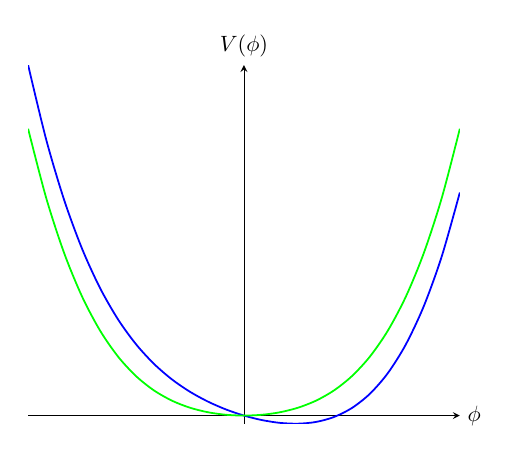
\begin{tikzpicture}[scale=0.8]
        \begin{axis} [axis lines=center, xtick=\empty, ytick=\empty, xlabel=$\phi$, ylabel=$V(\phi)$,
        every axis x label/.style={
            at={(ticklabel* cs:1.0)},
            anchor=west,
        },
        every axis y label/.style={
            at={(ticklabel* cs:1.0)},
            anchor=south,
        },]
            \addplot [domain=-3:3, smooth, thick, color=blue] { 6*x^2 + x^4 - 10*x };
            \addplot [domain=-3:3, smooth, thick, color=green] { 6*x^2 + x^4};
        \end{axis}
     
    \end{tikzpicture}
\end{minipage}
\hfill
\begin{minipage}{0.45\textwidth}
    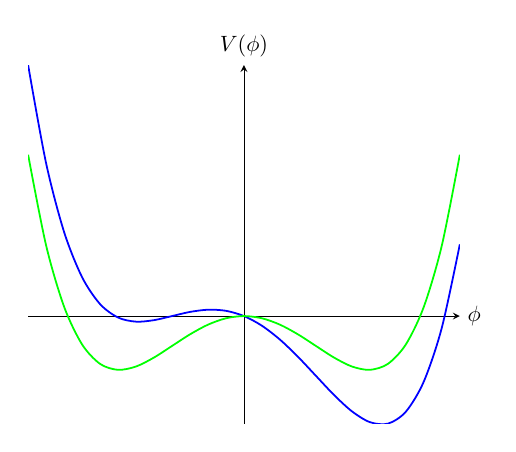
\begin{tikzpicture}[scale=0.8]
        \begin{axis} [axis lines=center, xtick=\empty, ytick=\empty, xlabel=$\phi$, ylabel=$V(\phi)$,
        every axis x label/.style={
            at={(ticklabel* cs:1.0)},
            anchor=west,
        },
        every axis y label/.style={
            at={(ticklabel* cs:1.0)},
            anchor=south,
        },]
            \addplot [domain=-3:3, smooth, thick, color=blue] { -6*x^2 + x^4 - 5*x };
            \addplot [domain=-3:3, smooth, thick, color=green] { -6*x^2 + x^4};
        \end{axis}
     
    \end{tikzpicture}
\end{minipage}
\label{fig:breaking_O1_symmetry}
\caption[Classical potential and symmetry breaking]{The introduction of the boson-fermion interaction, with a finite fermionic mass, causes explicit breaking of chiral symmetry, with consequence spontaneous breaking of the O(1) symmetry according to \eqref{eq:qualitative_relation_condensate_magnetisation}. It shifts the equilibrium position in the symmetric phase (left) causing $\left\langle \phi \right\rangle \neq 0$, and tilts the potential in the broken phase (right), making the two minima not equivalent.}
\end{figure}

\subsection{Phase structure and order parameters}
\begin{figure}
    \centering
    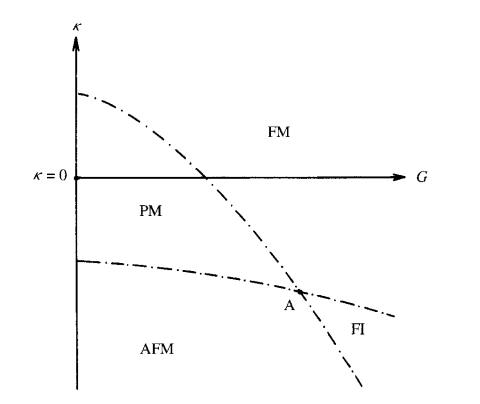
\includegraphics[scale=0.5]{figures/yukawa_phase_diagram.png}
    \caption[Yukawa phase diagram]{General phase diagram of a Yukawa theory. \\ \textcolor{blue}{I know that I wouldn't be allowed to use this picture, I will see later what to do.}}
    \label{fig:yukawa_phase_diagram}
\end{figure}
We want to conclude this chapter by commenting on the phase strcture of the Yukawa theory. This will guide the choice of parameters for the investigation carried in the remaining sections. A sketch of the different phases of the model is reported in figure \ref{fig:yukawa_phase_diagram}. 
The order parameters are the magnetisation $M = \expect{\phi}$ and the staggered magnetisation $M_s = \expect{\Phi}$, where
\begin{equation}
    {\Phi}_x \equiv(-1)^{t+x} \phi_x=\mathrm{e}^{\mathrm{i} \pi\left(t+x\right)} \phi_x .
\end{equation}
The four different phases are characterised by the following combinations of the order parameters
\begin{itemize}
    \item paramagnetic phase: $M = 0, M_s = 0$,
    \item ferromagnetic phase: $M \neq 0, M_s = 0$,
    \item anti-ferromagnetic phase: $M = 0, M_s \neq 0$,
    \item ferrimagnetic phase: $M \neq 0, M_s \neq 0$.
\end{itemize}
The lattice observables used for the investigation are introduced in section \ref{sec:observables}.